\section{Results and Discussions}
	%%%%%%%%%%%%%%%%%%%%%%%%%%%%%%%%%%%%%%%%%%%%%%%%%%%%%
	In this section we are going to show some results for delamination detection in accordance with a adaptive wavenumber filtering and a FCN-DenseNet model. 
	
	As we mentioned earlier, a sigmoid and a softmax functions are used at the output layer for our model, hence we have two versions of the FCN-DenseNet model with different output layer function.
	The sigmoid function at the output layer computes the damage probability for each pixel,hence the damage probability ranges from (\(0 - 1\)), therefore, there is a need for a threshold function to exclude low probabilities of predicted damage. 
	For all following results, the threshold \(tr = 0.5\), therefore any value less than \(0.5\) will be excluded from the damage map.
	For the softmax function at the output layer, it computes two probabilities for each pixel: [damaged and undamaged], then an \(argmax\) function is applied to select the highest probability between the two probabilities, therefore there is no need for thresholding. 
	The FCN-DenseNet models was trained on augmented dataset up to 100 epochs, and the architecture of the FCN-DenseNet  was implemented using the open-source platform of Keras API running on top of TensorFlow on a GeForce RTX 2080  GPU from NVIDIA.
	For all scenarios, we selected a red colour to represent the detected delamination (damaged), and the blue colour to represents the healthy state (undamaged).
	
	In the following, we are going to present three scenarios of full wavefield images with delaminations of different locations, shapes and angles.
	In fig.~\ref{fig:RMS_flat_shell_Vz_438} the full wavefield at bottom of the plate with delamination located at the top edge of the plate is shown, and fig.~\ref{fig:m1_rand_single_delam_438} shows its ground truth image. 
	Figs.~\ref{fig:ERMSF_flat_shell_Vz_438} shows the detected delamination using the adaptive wavenumber filtering, as seen the delamination is detected, but still there are some noise detected at the edges. 
	To exclude noise from the ERMSF a binary threshold is applied as shown in fig.~\ref{fig:Binary_ERMSF_flat_shell_Vz_438}, as shown from the binary ERMSF the delamination located, but still there is some noise at the corners, for this case the IoU = \(0.10\).
	In fig.~\ref{fig:predict_438_sigmoid_tr_0.5} and fig.~\ref{fig:predict_438_softmax} we present the FCN-DeneseNet outputs with sigmoid and softmax respectively.
	As shown, the FCN-DenseNet models only detected the delamination without any noise at the edges, due to the FCN-DenseNet learned the delamination patterns and can differentiate among different complex patterns such as noise.   
	The IoU = \(0.73\) for sigmoid, and IoU = \(0.65\) for the softmax.
	%%%%%%%%%%%%%%%%%%%%%%%%%%%%%%%%%%%%%%%%%%%%%%%%%%%
	%first figure
	%%%%%%%%%%%%%%%%%%%%%%%%%%%%%%%%%%%%%%%%%%%%%%%%%%%
	\begin{figure} [h!]
		\centering
		\begin{subfigure}[b]{0.47\textwidth}
			\centering
			\includegraphics[scale=1]{RMS_flat_shell_Vz_438_500x500bottom.png}
			\caption{RMS bottom}
			\label{fig:RMS_flat_shell_Vz_438}
		\end{subfigure}
		\hfill
			\begin{subfigure}[b]{0.47\textwidth}
			\centering
			\includegraphics[scale=1]{m1_rand_single_delam_438.png}
			\caption{Ground truth}
			\label{fig:m1_rand_single_delam_438}
		\end{subfigure}
		\hfill
		\begin{subfigure}[b]{0.47\textwidth}
			\centering
			\includegraphics[scale=1]{ERMSF_flat_shell_Vz_438_500x500bottom.png}
			\caption{ERMSF}
			\label{fig:ERMSF_flat_shell_Vz_438}
		\end{subfigure}
		\hfill
		\begin{subfigure}[b]{0.47\textwidth}
			\centering
			\includegraphics[scale=1]{Binary_ERMSF_flat_shell_Vz_438_500x500bottom.png}
			\caption{binary ERMSF}
			\label{fig:Binary_ERMSF_flat_shell_Vz_438}
		\end{subfigure}
		\hfill
		\begin{subfigure}[b]{0.47\textwidth}
			\centering
		\includegraphics[scale=1]{FCN_DenseNet_Predicted_438_sigmoid_thresholded_0.5.png}
		\caption{sigmoid \((tr = 0.5)\)}
		\label{fig:predict_438_sigmoid_tr_0.5}
		\end{subfigure}
		\hfill
		\begin{subfigure}[b]{0.47\textwidth}
			\centering
			\includegraphics[scale=1]{FCN_DenseNet_Predicted_438_softmax.png}
			\caption{softmax}
			\label{fig:predict_438_softmax}
		\end{subfigure}
		\caption{First scenario}
		\label{fig:RMS438}
	\end{figure} 
	%%%%%%%%%%%%%%%%%%%%%%%%%%%%%%%%%%%%%%%%%%%%%%%%%%%

	Fig.~\ref{fig:RMS454} presents the second scenario of a delamination located near the up left image.
	Fig.~\ref{fig:dispersion30deg_direct} and fig.~\ref{fig:m1_rand_single_delam_454} show the full wavefield at bottom of the plate with a delamination located at the up left of the image, and the ground truth image respectively.
	Fig.~\ref{fig:ERMSF_flat_shell_Vz_454} shows the detected delamination using the adaptive wavenumber filtering.
	As shown for adaptive filtering it still depict some noise at the edges, therefore, binary thresholding was applied as shown in fig.~\ref{fig:Binary_ERMSF}, the IoU for this case is \(0.61\).
	In fig.~\ref{fig:predict_454_sigmoid_tr_0.5} and fig.~\ref{fig:predict_454_softmax} we present the FCN-DeneseNet outputs with sigmoid and softmax respectively.
	The sigmoid detect the delamination with IoU = \(0.58\), and for the softmax with IoU = \(0.60\).
	As we can see also for this scenario, the FCN-DenseNet only detects the delamination patterns.
	%%%%%%%%%%%%%%%%%%%%%%%%%%%%%%%%%%%%%%%%%%%%%%%%%%%
	\begin{figure} [h!]
		\centering
		\begin{subfigure}[b]{0.47\textwidth}
			\centering
			\includegraphics[scale=1]{RMS_flat_shell_Vz_454_500x500bottom.png}
			\caption{RMS bottom}
			\label{fig:dispersion30deg_direct}
		\end{subfigure}
		\hfill
		\begin{subfigure}[b]{0.47\textwidth}
			\centering
			\includegraphics[scale=1]{m1_rand_single_delam_454.png}
			\caption{Ground truth}
			\label{fig:m1_rand_single_delam_454}
		\end{subfigure}
		\hfill
		\begin{subfigure}[b]{0.47\textwidth}
			\centering
			\includegraphics[scale=1]{ERMSF_flat_shell_Vz_454_500x500bottom.png}
			\caption{ERMSF}
			\label{fig:ERMSF_flat_shell_Vz_454}
		\end{subfigure}
		\hfill
		\begin{subfigure}[b]{0.47\textwidth}
			\centering
			\includegraphics[scale=1]{Binary_ERMSF_flat_shell_Vz_454_500x500bottom.png}
			\caption{Binary ERMSF}
			\label{fig:Binary_ERMSF}
		\end{subfigure}
		\hfill
		\begin{subfigure}[b]{0.47\textwidth}
			\centering
			\includegraphics[scale=1]{FCN_DenseNet_Predicted_454_sigmoid_thresholded_0.5.png}
			\caption{sigmoid (tr =\(0.5\))}
			\label{fig:predict_454_sigmoid_tr_0.5}
		\end{subfigure}
		\hfill	
		\begin{subfigure}[b]{0.47\textwidth}
			\centering
			\includegraphics[scale=1]{FCN_DenseNet_Predicted_454_softmax.png}
			\caption{softmax}
			\label{fig:predict_454_softmax}
		\end{subfigure}
		\caption{Second scenario}
		\label{fig:RMS454}
	\end{figure} 
	%%%%%%%%%%%%%%%%%%%%%%%%%%%%%%%%%%%%%%%%%%%%%%%%%%%

	In fig.~\ref{fig:RMS433} we present the third scenario where the adaptive wavenumber filtering can detect the delamination whereas the FCN-DenseNet model failed.
	As shown in fig.~\ref{fig:RMS_flat_shell_Vz_433} the full wavefield at bottom of the plate with a delamination located at the upper left corner of the image
	and the delamination ground truth can be seen in fig.~\ref{fig:m1_rand_single_delam_433}. 
	As shown in fig.~\ref{fig:ERMSF_flat_shell_Vz_433} the detected delamination using the adaptive filtering, fig.~\ref{fig:Binary_ERMSF_flat_shell_Vz_433} the binary thresholded ERMSF. 
	Delaminations located near edges or corners are difficult to detect due to reflected waves have similar patterns for both conventional and deep learning techniques. 
	However, to solve this issue for the FCN model, we need to enhance the feature extraction process by obtaining more data to train the model to recognize and learn new patterns.	
	%%%%%%%%%%%%%%%%%%%%%%%%%%%%%%%%%%%%%%%%%%%%%%%%%%%
	% third figure
	%%%%%%%%%%%%%%%%%%%%%%%%%%%%%%%%%%%%%%%%%%%%%%%%%%%
	\begin{figure} [h!]
		\centering
		\begin{subfigure}[b]{0.47\textwidth}
			\centering
			\includegraphics[scale=1]{RMS_flat_shell_Vz_433_500x500bottom.png}
			\caption{RMS bottom}
			\label{fig:RMS_flat_shell_Vz_433}
		\end{subfigure}
		\hfill
		\begin{subfigure}[b]{0.47\textwidth}
			\centering
			\includegraphics[scale=1]{m1_rand_single_delam_433.png}
			\caption{ground truth}
			\label{fig:m1_rand_single_delam_433}
		\end{subfigure}
		\hfill
		\begin{subfigure}[b]{0.47\textwidth}
			\centering
			\includegraphics[scale=1]{ERMSF_flat_shell_Vz_433_500x500bottom.png}
			\caption{ERMSF}
			\label{fig:ERMSF_flat_shell_Vz_433}
		\end{subfigure}
		\hfill
		\begin{subfigure}[b]{0.47\textwidth}
			\centering
			\includegraphics[scale=1]{Binary_ERMSF_flat_shell_Vz_433_500x500bottom.png}
			\caption{binary ERMSF}
			\label{fig:Binary_ERMSF_flat_shell_Vz_433}
		\end{subfigure}
		
		%	\begin{subfigure}[b]{0.47\textwidth}
		%		\centering
		%		\includegraphics[scale=1]{FCN_DenseNet_Predicted_433_sigmoid_thresholded_0.1.png}
		%		\caption{sigmoid,n(433), tr (0.1)}
		%		\label{fig:predict_433_sigmoid_tr_0.1}
		%	\end{subfigure}
		
		%		\begin{subfigure}[b]{0.47\textwidth}
		%			\centering
		%			\includegraphics[scale=1]{FCN_DenseNet_Predicted_433_softmax.png}
		%			\caption{softmax, n(433)}
		%			\label{fig:predict_433_softmax}
		%		\end{subfigure}
		\caption{Third scenario}
		\label{fig:RMS433}
	\end{figure} 
	In table~\ref{tab:iou} we present the (maximum, minimum and mean) IoU for the adaptive filtering and FCN-DenseNet for sigmoid and softmax for all testing images.
	\begin{table}
		\centering
		\caption{IoU for all models, sigmoid at threshold = 0.5}
		\label{tab:iou}
		\resizebox{\textwidth}{!}{\begin{tabular}{ccccccccccccc}
				\hline
				&  &  &  &  &  & \multicolumn{7}{c}{FCN-Dense Model} \\ \cline{7-13} 
				&  & \multicolumn{3}{c}{Adaptive filtering} &  & \multicolumn{3}{c}{sigmoid} &  & \multicolumn{3}{c}{softmax} \\ \cline{3-5} \cline{7-9} \cline{11-13} 
				&  & minimum & maximum & mean &  & minimum & maximum & mean &  & \multicolumn{1}{c}{minimum} & \multicolumn{1}{c}{maximum} & \multicolumn{1}{c}{mean} \\ \cline{3-13} 
				\multicolumn{2}{c}{IoU} &0&0.648&0.373& &0&0.933&0.616&  &0&0.878&0.623\\ 
				\hline
		\end{tabular}}
	\end{table}

	In fig.~\ref{fig:Exp_ERMS_teflon} we present an experimental scenario, of CFRP with Teflon inserted and a frequency of \(50 Hz\) is used to excite the transducer.
	As shown if fig.~\ref{fig:ERMSF_CFRP_teflon} the adaptive filtering is able to detect the delamination and fig.~\ref{fig:Binary_ERMSF_CFRP} shows the binary thresholded output. 
	The FCN-DesneNet model detected the delamination with both a sigmoid and softmax functions in fig.~\ref{fig:EXP_predict_sigmoid} and fig.~\ref{fig:EXP_predict_softmax} respectively.
	\begin{figure} [h!]
		\centering
		\begin{subfigure}[b]{0.47\textwidth}
			\centering
			\includegraphics[scale=1]{ERMS_CFRP_teflon_3o_375_375p_50kHz_5HC_x12_15Vpp.png}
			\caption{ERMS CFRP Teflon inserted}
			\label{fig:Delamination}
		\end{subfigure}			
		\hfill
		\begin{subfigure}[b]{0.47\textwidth}
			\centering 	
			\includegraphics[scale=1]{label_CFRP_teflon_3o_375_375p_50kHz_5HC_x12_15Vpp.png}
			\caption{Ground truth} 
			\label{fig:damage_label}
		\end{subfigure}
		\hfill
		\begin{subfigure}[b]{0.47\textwidth}
			\centering
			\includegraphics[scale=1]{ERMSF_CFRP_teflon_3o_375_375p_50kHz_5HC_x12_15Vpp.png}
			\caption{ERMSF} 
			\label{fig:ERMSF_CFRP_teflon}
		\end{subfigure}
		\hfill
		\begin{subfigure}[b]{0.47\textwidth}
		\centering
		\includegraphics[scale=1]{Binary_ERMSF_CFRP_teflon_3o_375_375p_50kHz_5HC_x12_15Vpp.png}
		\caption{Binary ERMSF} 
		\label{fig:Binary_ERMSF_CFRP}
		\end{subfigure}
		\hfill
		\begin{subfigure}[b]{0.47\textwidth}
			\centering
			\includegraphics[scale=1]{Predicted_Predicted_ERMS_CFRP_teflon_3o_375_375p_50kHz_5HC_x12_15Vpp_7__threshold_0.5_sigmoid.png}
			\caption{FCN DenseNet: sigmoid \((tr = 0.5)\)} 
			\label{fig:EXP_predict_sigmoid}
		\end{subfigure}
		\hfill
		\begin{subfigure}[b]{0.47\textwidth}
			\centering
			\includegraphics[scale=1]{Predicted_Predicted_ERMS_CFRP_teflon_3o_375_375p_50kHz_5HC_x12_15Vpp_7_softmax.png}
			\caption{FCN DenseNet: softmax} 
			\label{fig:EXP_predict_softmax}
		\end{subfigure}
			\caption{Experimental results}
			\label{fig:Exp_ERMS_teflon}
		\end{figure}
	
	Every single value of the IoU was estimated for all testing images using FCN-DenseNet with a sigmoid at the output layers.
	It is expected that as we increase the threshold the IoU will decrease due to some of the detected output values will be excluded, therefore, selecting the proper threshold value is important for maximizing IoU. Fig.~\ref{fig:iou_fcn} shows how IoU is decreasing along with the threshold increment in the range of \(0-1\) with a step value of \(0.01\).
	\begin{figure}
		\centering
		\includegraphics[width=\textwidth]{fcn_densenet_iou.png}
		\centering
		\caption{IoU for FCN-DenseNet with sigmoid of a range of thresholds \([0-1]\)} 
		\label{fig:iou_fcn}
	\end{figure}
%%%%%%%%%%%%%%%%%%%%%%

	
